\documentclass[aspectratio=169]{beamer}
%
% Choose how your presentation looks.
%
% For more themes, color themes and font themes, see:
% http://deic.uab.es/~iblanes/beamer_gallery/index_by_theme.html
%
\mode<presentation>
{
  \usetheme{metropolis}      % or try Darmstadt, Madrid, Warsaw, ...
  \usecolortheme{default} % or try albatross, beaver, crane, ...
  \usefonttheme{structurebold}  % or try serif, structurebold, ...
  \setbeamercolor{background canvas}{bg=white}
  \setbeamertemplate{navigation symbols}{}
  \setbeamertemplate{bibliography item}{\insertbiblabel}
  %\setbeamertemplate{caption}[numbered]
} 
\usepackage[english]{babel}
\usepackage[utf8x]{inputenc}
\usepackage{listings}             % Include the listings-package
\hypersetup{
    colorlinks = true,
    linkcolor = {black},
    urlcolor = {blue}
}
\usepackage{animate}

\DeclareMathOperator*{\argmin}{arg\,min}

\title[Deep Learning and Temporal Data Processing]{Deep Learning and Temporal Data Processing}
\subtitle{2 - Convolutional Neural Networks}
\institute{University of Modena and Reggio Emilia}
\author{Andrea Palazzi}
\date{June 21th, 2017}

\def\thisframelogos{}

\newcommand{\framelogo}[1]{\def\thisframelogos{#1}}

\addtobeamertemplate{frametitle}{}{%
\begin{tikzpicture}[remember picture,overlay]
\node[anchor=north east] at (current page.north east) {%
    \foreach \img in \thisframelogos {%
        %\hspace{.5ex}%
        \includegraphics[height=3.5ex]{\img}%
    }%
};
\end{tikzpicture}}

\begin{document}

\framelogo{logo_unimore_white.png}

\bgroup
\renewcommand{\insertframenumber}{}
\begin{frame}[noframenumbering]
  \titlepage
\end{frame}
\egroup
\begin{frame}{Agenda}
  \tableofcontents
\end{frame}



%%%%%%%%%%%%%%%%%%%%%%%%%%%%%%%%%%%%%%%%%%%%%%%%%%%%%%%%%%%%%%%%%%
%%%%%%%%%%%%%%%%%%%%%%%%%%%%%%%%%%%%%%%%%%%%%%%%%%%%%%%%%%%%%%%%%%
%%%%%%%%%%%%%%%%%%%%%%%%%%%%%%%%%%%%%%%%%%%%%%%%%%%%%%%%%%%%%%%%%%


\section{Introduction}

%%%%%%%%%%%%%%%%%%%%%%%%%%%%%%%%%%%%%%%%%%%%%%%%%%%%%%%%%%%%%%%%%%

\begin{frame}{CNNs: overview}
Convolutional Neural Networks are very similar to ordinary Neural Networks.\\
\begin{itemize}
\item They are made up of neurons that have learnable weights and biases.
\item Each neuron receives some inputs, performs a dot product and optionally follows it with a non-linearity.
\item The whole network still expresses a single differentiable function.
\end{itemize}
\end{frame}

%%%%%%%%%%%%%%%%%%%%%%%%%%%%%%%%%%%%%%%%%%%%%%%%%%%%%%%%%%%%%%%%%%

\begin{frame}{CNNs: overview}
However, \textbf{CNNs make the explicit assumption that inputs are images}.
\begin{itemize}
\item \large{This architecture constraint paves the way to more efficient implementation, better performance and a vastly reduced amount of learnable parameters \emph{w.r.t.} fully-connected deep networks.}
\end{itemize}
Most important peculiarities of CNNs are presented in the following slides.
\end{frame}


%%%%%%%%%%%%%%%%%%%%%%%%%%%%%%%%%%%%%%%%%%%%%%%%%%%%%%%%%%%%%%%%%%
%%%%%%%%%%%%%%%%%%%%%%%%%%%%%%%%%%%%%%%%%%%%%%%%%%%%%%%%%%%%%%%%%%
%%%%%%%%%%%%%%%%%%%%%%%%%%%%%%%%%%%%%%%%%%%%%%%%%%%%%%%%%%%%%%%%%%


\section{Architecture}

\begin{frame}{CNN Architecture}
Unlike a regular neural network, CNN layers have neurons arranged in 3 dimensions: width ($W$), height ($H$) and depth ($C$).
\begin{figure}
\begin{tabular}{c}
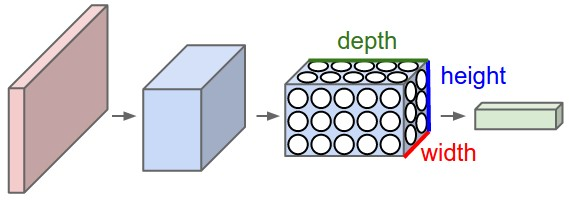
\includegraphics[width=0.5\textwidth]{img/cnn/cnn_vs_dnn.jpg}
\end{tabular}
\end{figure}

\textbf{Achtung}: in the following we'll refer to the word \emph{depth} to indicate the number of channels of an activation volume. This has nothing to do with the depth of the whole network, which usually refers to the total number of layers in the network.
\end{frame}

%%%%%%%%%%%%%%%%%%%%%%%%%%%%%%%%%%%%%%%%%%%%%%%%%%%%%%%%%%%%%%%%%%

\begin{frame}{CNN Architecture}
An "real-world" CNN is made up by a whole bunch of layers stacked one on the top of the other.
\begin{figure}
\begin{tabular}{c}
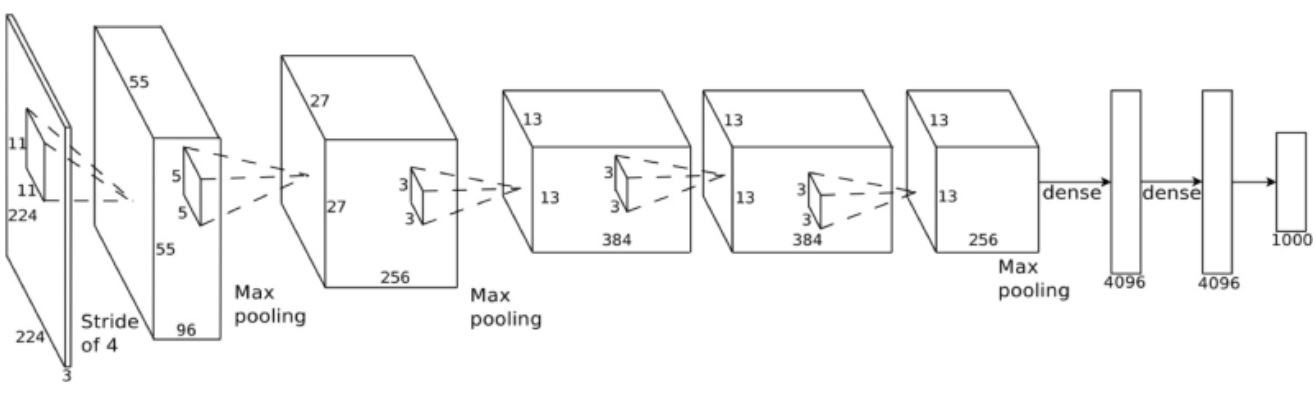
\includegraphics[width=0.6\textwidth]{img/cnn/cnn_architecture.jpg}
\end{tabular}
\end{figure}
\large{Every layer has a simple API: \emph{it transforms an input 3D volume to an output 3D volume with some differentiable function that may or may not have parameters}}.
\end{frame}

%%%%%%%%%%%%%%%%%%%%%%%%%%%%%%%%%%%%%%%%%%%%%%%%%%%%%%%%%%%%%%%%%%

\begin{frame}{Convolutional Layers}
The \textbf{Convolutional Layer} is the core building block of convolutional neural networks.\\
\vspace{0.2cm}
\textbf{Intuition}: every convolutional layer is equipped with a set of learnable filters. During the forward pass, each filter is convolved with the input volume thus producing a 2D activation map. One map for each filter is produced. The output volume is then made up by stacking all activation maps produced one on the top of the other. 	
\begin{figure}
\begin{tabular}{c}
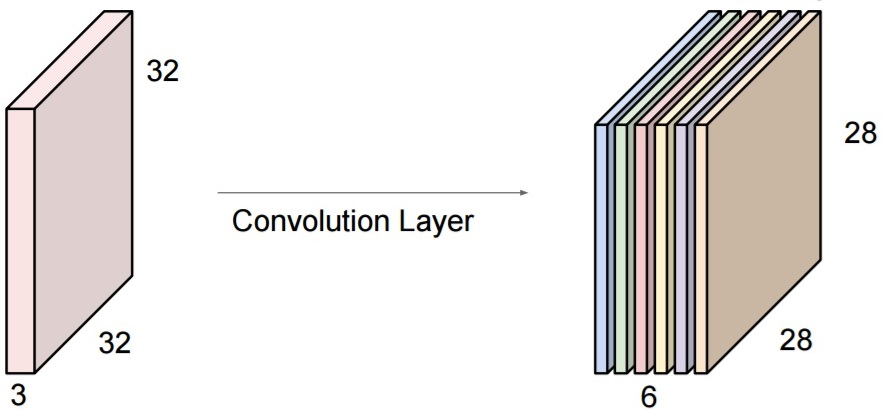
\includegraphics[width=0.4\textwidth]{img/cnn/activation_maps.jpg}\\
\small{\emph{e.g.} Result of $N=6$ filters of kernel size $K=5$x$5$ convolved on input image.}
\end{tabular}
\end{figure}
\end{frame}

%%%%%%%%%%%%%%%%%%%%%%%%%%%%%%%%%%%%%%%%%%%%%%%%%%%%%%%%%%%%%%%%%%

\begin{frame}{Convolutional Layers}
Each convolutional layer has three main hyperparameters:
\begin{itemize}
\item Number of filters $N$
\item Kernel size $K$, the spatial size of the filters convolved
\item Filter stride $S$, factor by which to downscale
\end{itemize}
The presence and amount of spatial padding $P$ on the input volume may be considered an additional hyperparameter. In practice padding is usually performed to avoid headaches caused by convolutions "eating the borders".
\end{frame}

%%%%%%%%%%%%%%%%%%%%%%%%%%%%%%%%%%%%%%%%%%%%%%%%%%%%%%%%%%%%%%%%%%

\begin{frame}{Visualizing Convolution 2D}
\begin{figure}
\begin{tabular}{c}
Convolution 2D, half padding, stride $S=1$.\\
  \animategraphics[loop,controls,width=0.35\textwidth]{1}{img/cnn/conv_animation/conv_animation-}{0}{24}
\end{tabular}
\end{figure}
\end{frame}

%%%%%%%%%%%%%%%%%%%%%%%%%%%%%%%%%%%%%%%%%%%%%%%%%%%%%%%%%%%%%%%%%%

\begin{frame}{Visualizing Convolution 2D}
\begin{figure}
\begin{tabular}{c}
Convolution 2D, no padding, stride $S=2$.\\
  \animategraphics[loop,controls,width=0.35\textwidth]{1}{img/cnn/conv_animation_stride/conv_animation_stride-}{0}{3}
\end{tabular}
\end{figure}
\end{frame}

%%%%%%%%%%%%%%%%%%%%%%%%%%%%%%%%%%%%%%%%%%%%%%%%%%%%%%%%%%%%%%%%%%

\begin{frame}{Convolutional Layers: Local Connectivity}
Looking closer, neurons in a CNN perform the very same operation of the neurons we already know from DNN.
\begin{equation*}
		\sum_i w_i x_i + b
\end{equation*}
\begin{columns}
    \begin{column}{0.48\textwidth}
    \centering
		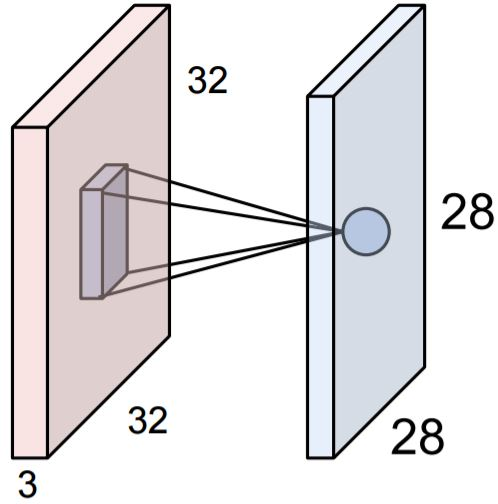
\includegraphics[width=0.5\textwidth]{img/cnn/local_connectivity.jpg}
    \end{column}
     \begin{column}{0.48\textwidth}
However, in convolutional layers neurons are only locally connected to the input volume. The small region that each neuron "sees" of the previous layer is usually referred to as the \textit{receptive field} of the neuron.
    \end{column}
\end{columns}
\end{frame}

%%%%%%%%%%%%%%%%%%%%%%%%%%%%%%%%%%%%%%%%%%%%%%%%%%%%%%%%%%%%%%%%%%

\begin{frame}{Convolutional Layers: Parameter Sharing}
Assumption: if a feature is useful to compute at some spatial location $(x,y)$, then it should be useful to compute also at different locations $(x_i,y_i)$. \textbf{Thus, we constrain the neurons in each depth slice to use the same weights and bias.}

If all neurons in a single depth slice are using the same weight vector, then the forward pass of the convolutional layer can \emph{in each depth slice} be computed as a convolution of the neuron’s weights with the input volume (hence the name). This is why it is common to refer to each set of weights as a filter (or a kernel), that is convolved with the input.
\end{frame}

%%%%%%%%%%%%%%%%%%%%%%%%%%%%%%%%%%%%%%%%%%%%%%%%%%%%%%%%%%%%%%%%%%

\begin{frame}{Convolutional Layers: Parameter Sharing}
\begin{figure}
\begin{tabular}{c}
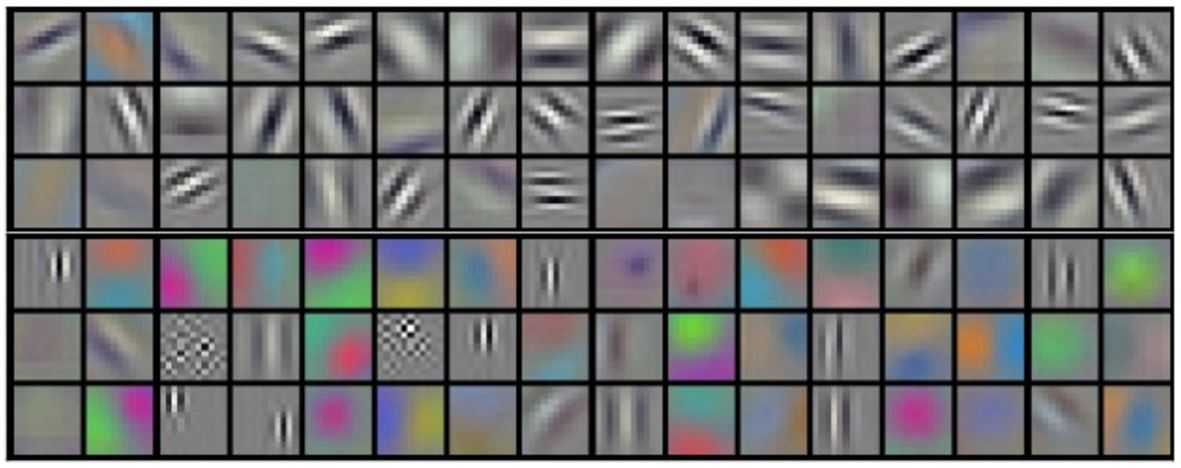
\includegraphics[width=0.80\textwidth]{img/cnn/learned_weights.jpg}
\end{tabular}
\end{figure}
\small{Example of weights learned by \cite{krizhevsky2012imagenet}. Each of the 96 filters shown here is of size [11x11x3], and each one is shared by the 55*55 neurons in one depth slice. Notice that the parameter sharing assumption is relatively reasonable: If detecting a horizontal edge is important at some location in the image, it should intuitively be useful at some other location as well due to the translationally-invariant structure of images.}
\end{frame}

%%%%%%%%%%%%%%%%%%%%%%%%%%%%%%%%%%%%%%%%%%%%%%%%%%%%%%%%%%%%%%%%%%

\begin{frame}{Convolutional Layers: Number of Learnable Parameters}
Given an input volume of size $H_1$ x $W_1$ x $C_1$, the number of \textbf{learnable parameters} of a convolutional layer with $N$ filters and kernel size $K$x$K$ is:
\begin{equation*}
tot\_learnable = N * K * K * C_1 + N
\end{equation*}
\small{\textit{Explanation}: there are N filters which convolve on input volume. The neural connection is local on width and height, but extends for the full depth of input volume, so there are $K * K * C_1$ parameters for each filter. Furthermore, each filter has an additive learnable bias.}
\end{frame}

%%%%%%%%%%%%%%%%%%%%%%%%%%%%%%%%%%%%%%%%%%%%%%%%%%%%%%%%%%%%%%%%%%

\begin{frame}{Pooling Layers: overview}
Pooling layers spatially subsample the input volume.\\
Each depth slice of the input is processed independently.\\
\begin{figure}
\begin{tabular}{c}
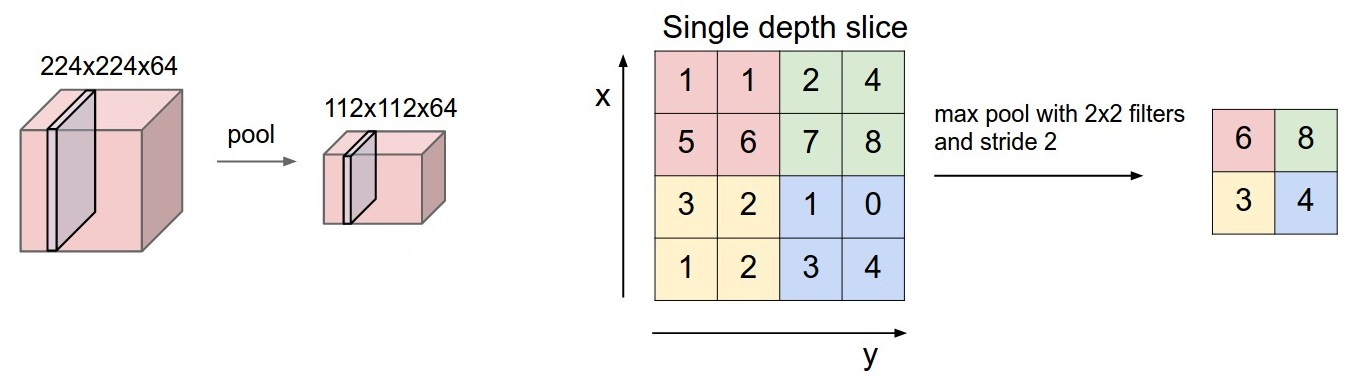
\includegraphics[width=0.90\textwidth]{img/cnn/pool.jpg}
\end{tabular}
\end{figure}
Two hyperparameters:
\begin{itemize}
\item Pool size $K$, which is the size of the pooling window
\item Pool stride $S$, which is the factor by which to downscale
\end{itemize}
%\begin{equation*}
%A_{i,j} = e^{-\frac{\sum_{k=1}^d||x_i^k-x_j^k||^2}{\sigma^2}}
%\end{equation*}
\end{frame}

%%%%%%%%%%%%%%%%%%%%%%%%%%%%%%%%%%%%%%%%%%%%%%%%%%%%%%%%%%%%%%%%%%

\begin{frame}{Pooling Layers: types}
The pooling function may be considered an additional hyperparameter.

In principle, many different functions could be used.

In practice, the \textbf{max} pooling is by far the most common
\begin{equation*}
h^n_i(x, y) = max_{\bar{x},\bar{y} \in N(x, y)}h^{n-1}_{i}(\bar{x},\bar{y})
\end{equation*}
Another common pooling function is the \textbf{average}
\begin{equation*}
h^n_i(x, y) = \frac{1}{K}\sum_{\bar{x},\bar{y} \in N(x, y)}h^{n-1}_{i}(\bar{x},\bar{y})
\end{equation*}
\end{frame}

%%%%%%%%%%%%%%%%%%%%%%%%%%%%%%%%%%%%%%%%%%%%%%%%%%%%%%%%%%%%%%%%%%

\begin{frame}{Pooling Layers: why}
Pooling layers are widely used for a number of reasons:
\begin{itemize}
\item Gain robustness to exact location of the features
\item Reduce computational (memory) cost
\item Help preventing overfitting
\item Increase receptive field of following layers
\end{itemize}
Most common configuration: pool size $K=2$x$2$, stride $S=2$.\\
In this setting 75\% of input volume activations are discarded.
\end{frame}

%%%%%%%%%%%%%%%%%%%%%%%%%%%%%%%%%%%%%%%%%%%%%%%%%%%%%%%%%%%%%%%%%%

\begin{frame}{Pooling Layers: why not}
The loss of spatial resolution is not always beneficial.\\
\emph{e.g.} semantic segmentation
\begin{figure}
\begin{tabular}{cc}
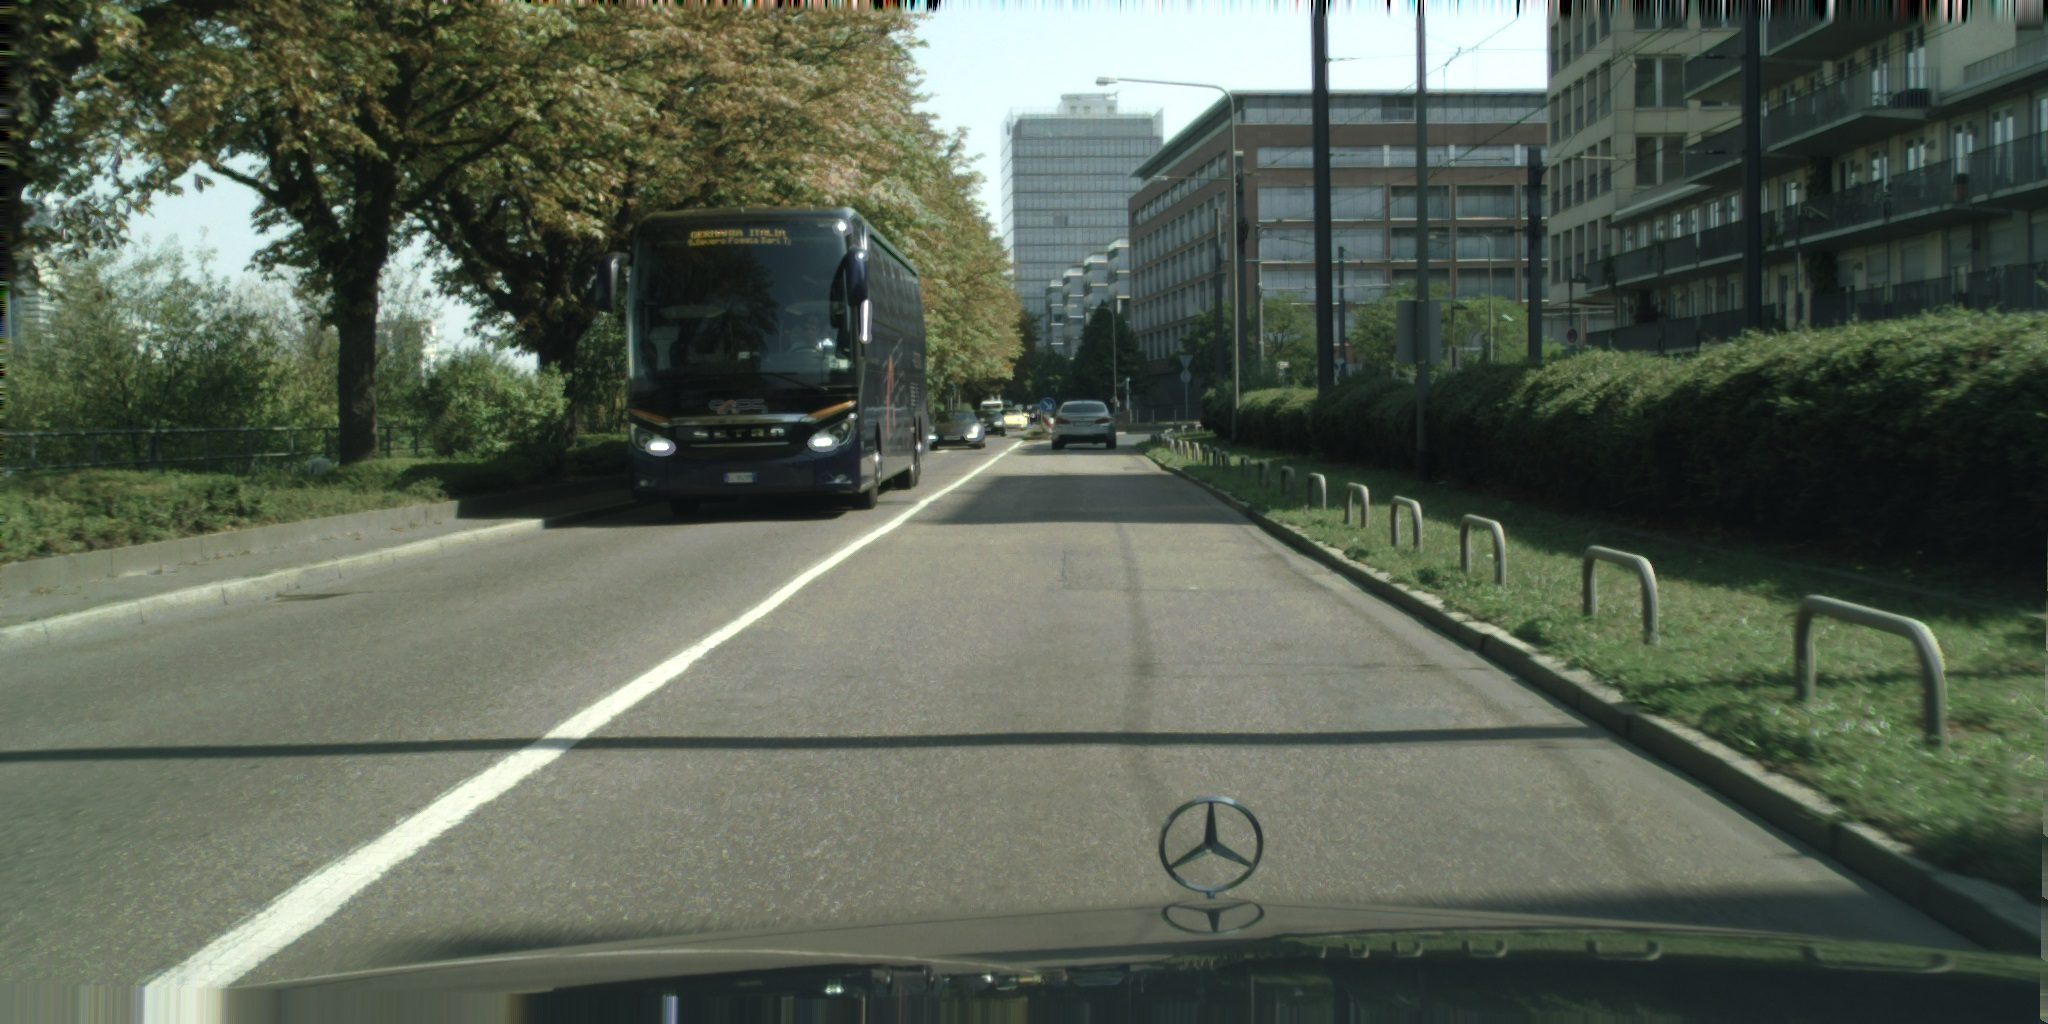
\includegraphics[width=0.3\textwidth]{img/cnn/semseg_in.jpg}&
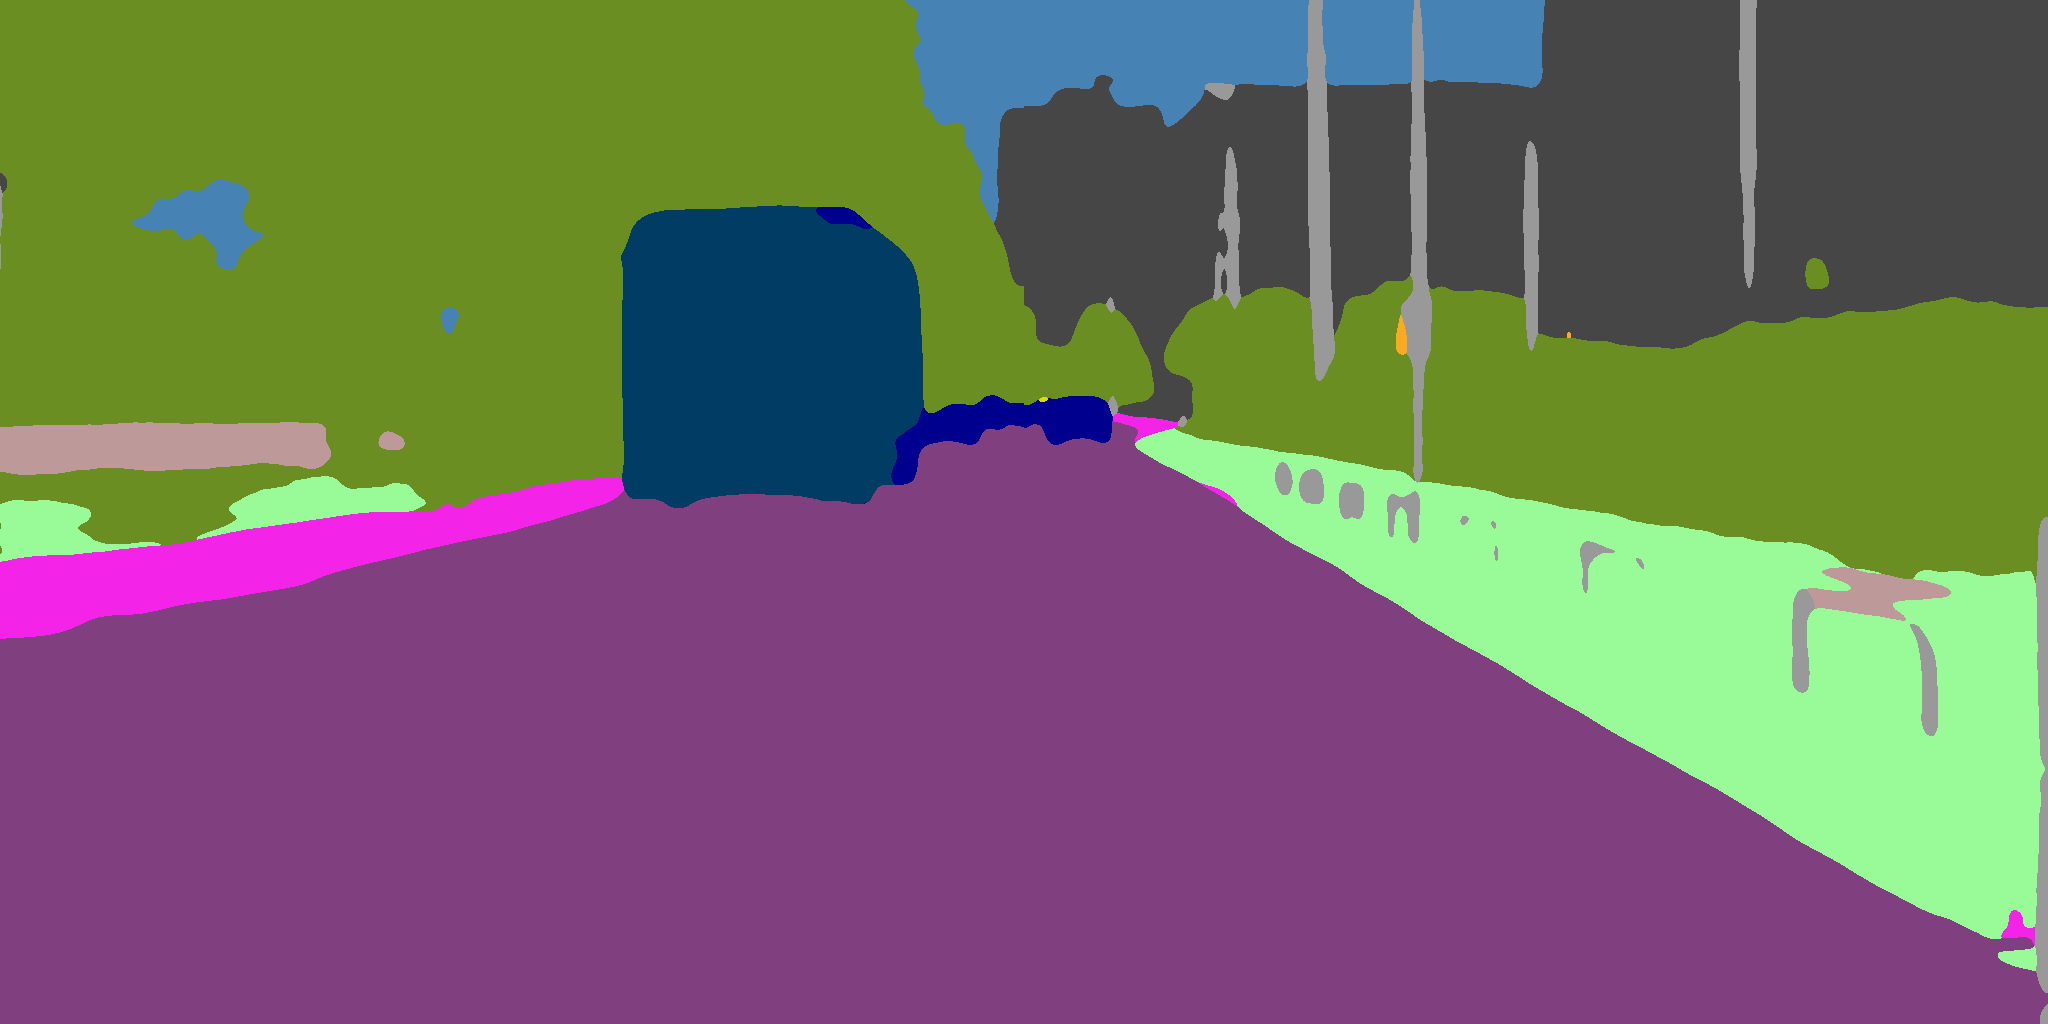
\includegraphics[width=0.3\textwidth]{img/cnn/semseg_out.png}
\end{tabular}
\end{figure}
There's a lot of research on getting rid of pooling layers while mantaining the benefits (\emph{e.g.} \cite{springenberg2014striving,yu2015multi}). We'll see if future architecture will still feature pooling layers.
\end{frame}

%%%%%%%%%%%%%%%%%%%%%%%%%%%%%%%%%%%%%%%%%%%%%%%%%%%%%%%%%%%%%%%%%%

\begin{frame}{Activation Layers}

Activation layers compute non-linear activation function elementwise on the input volume. The most common activations are \textbf{ReLu}, \textbf{sigmoid} and \textbf{tanh}.
\begin{figure}
\begin{tabular}{ccc}
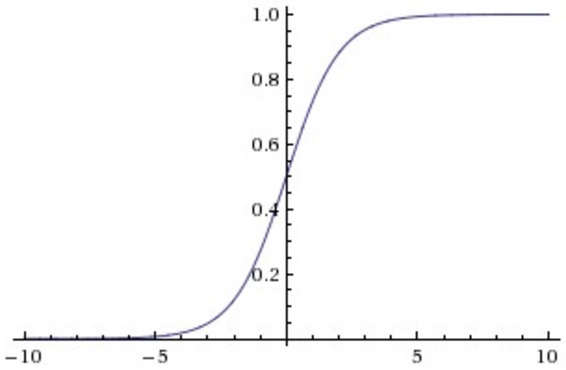
\includegraphics[width=0.3\textwidth]{img/cnn/act_sigmoid.jpg}&
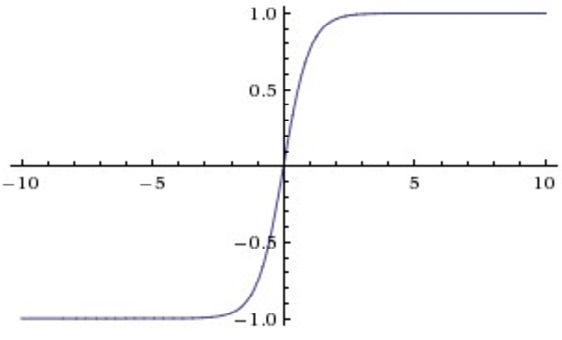
\includegraphics[width=0.3\textwidth]{img/cnn/act_tanh.jpg} & 
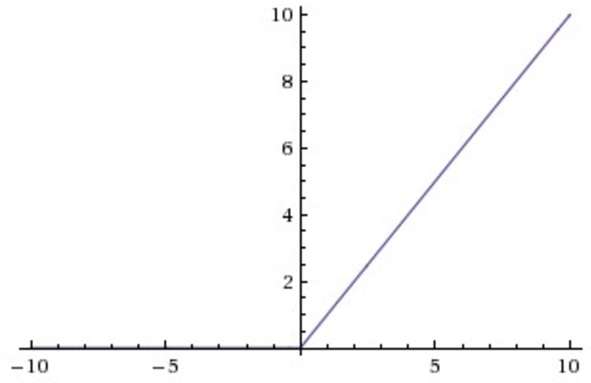
\includegraphics[width=0.3\textwidth]{img/cnn/act_relu.jpg}\\
Sigmoid & Tanh & ReLu
\end{tabular}
\end{figure}
Nonetheless, more complex activation functions exist \cite{he2015delving,goodfellow2013maxout}.
\end{frame}

%%%%%%%%%%%%%%%%%%%%%%%%%%%%%%%%%%%%%%%%%%%%%%%%%%%%%%%%%%%%%%%%%%

\begin{frame}{Activation Layers}
\textbf{ReLu wins}\\
ReLu was found to greatly accelerate the convergence of SGD compared to sigmoid/tanh functions \cite{krizhevsky2012imagenet}. Furthermore, ReLu can be implemented by a simple threshold, \emph{w.r.t.} other activations which require complex operations.

\textbf{Why using non-linear activations at all?}\\
Composition of linear functions is a linear function. Without nonlinearities, neural networks would reduce to 1 layer logistic regression.

\end{frame}

%%%%%%%%%%%%%%%%%%%%%%%%%%%%%%%%%%%%%%%%%%%%%%%%%%%%%%%%%%%%%%%%%%

\begin{frame}{Computing Output Volume Size}
\textbf{Convolutional layer}: given an input volume of size $H_1$ x $W_1$ x $C_1$, the output of a convolutional layer with $N$ filters, kernel size $K$, stride $S$ and zero padding $P$ is a volume with new shape $H_2$ x $W_2$ x $C_2$, where:
\begin{itemize}
\item $H_2 = (H_1 - K + 2P) / S + 1$ 
\item $W_2 = (W_1 - K + 2P) / S + 1$ 
\item $C_2 = N$
\end{itemize}
\end{frame}

%%%%%%%%%%%%%%%%%%%%%%%%%%%%%%%%%%%%%%%%%%%%%%%%%%%%%%%%%%%%%%%%%%

\begin{frame}{Computing Output Volume Size}
\textbf{Pooling layer}: given an input volume of size $H_1$ x $W_1$ x $C_1$, the output of a pooling layer with pool size $K$ and pool stride $S$ is a volume with new shape $H_2$ x $W_2$ x $C_2$, where:
\begin{itemize}
\item $H_2 = (H_1 - K) / S + 1$ 
\item $W_2 = (W_1 - K) / S + 1$ 
\item $C_2 = C_1$
\end{itemize}
\textbf{Activation layer}: given an input volume of size $H_1$ x $W_1$ x $C_1$, the output of an activation layer is a volume with shape $H_2$ x $W_2$ x $C_2$, where:
\begin{itemize}
\item $H_2 = H_1$ 
\item $W_2 = W_1$ 
\item $C_2 = C_1$
\end{itemize}
\end{frame}

%%%%%%%%%%%%%%%%%%%%%%%%%%%%%%%%%%%%%%%%%%%%%%%%%%%%%%%%%%%%%%%%%%

\begin{frame}{Advanced CNN Architectures}
More complex CNN architectures have recently been demonstrated to perform better than the traditional \texttt{conv -> relu -> pool } stack architecture.

These architectures usually feature different graph topologies and much more intricate connectivity structures (\emph{e.g.} \cite{he2016deep,szegedy2016rethinking}).

However, these advanced architectures are out of the scope of these lectures.
\end{frame}

%%%%%%%%%%%%%%%%%%%%%%%%%%%%%%%%%%%%%%%%%%%%%%%%%%%%%%%%%%%%%%%%%%

\begin{frame}{Computational Footprint}
If we consider a standard convolutional network like VGG \cite{simonyan2014very} we can make a couple of considerations on the computational footprint.
\begin{figure}
\begin{tabular}{c}
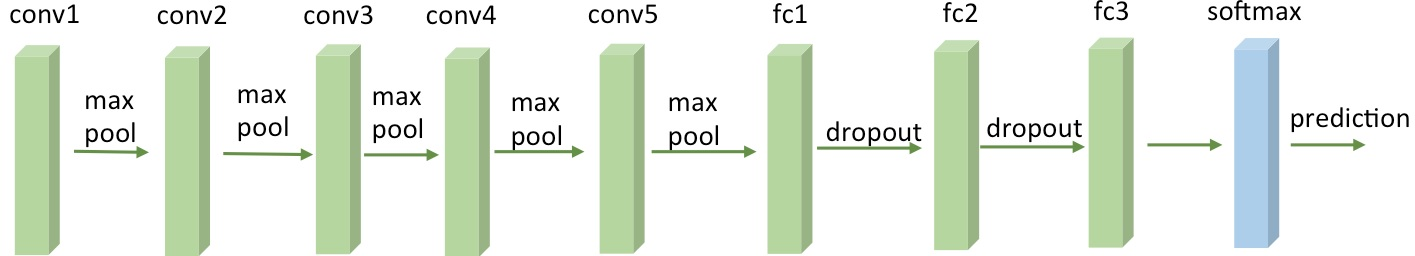
\includegraphics[width=0.8\textwidth]{img/cnn/vgg16.jpg}
\end{tabular}
\end{figure}
\begin{itemize}
\item Most of the memory is taken by the very first layers
\item Most of parameters (70\%) are condensated in the last fully-connected layers
\end{itemize}
\small{Can you justify why?}
\end{frame}

%%%%%%%%%%%%%%%%%%%%%%%%%%%%%%%%%%%%%%%%%%%%%%%%%%%%%%%%%%%%%%%%%%

%\begin{frame}{Troubleshooting}
%\begin{itemize}
%\item Check gradient numerically by finite differences:
%\begin{equation*}
%f'(x) = \frac{f(x+\epsilon) - f(x-\epsilon)}{2\epsilon}
%\end{equation*}
%\end{itemize}
%\end{frame}

%%%%%%%%%%%%%%%%%%%%%%%%%%%%%%%%%%%%%%%%%%%%%%%%%%%%%%%%%%%%%%%%%%

%%%%%%%%%%%%%%%%%%%%%%%%%%%%%%%%%%%%%%%%%%%%%%%%%%%%%%%%%%%%%%%%%%
%%%%%%%%%%%%%%%%%%%%%%%%%%%%%%%%%%%%%%%%%%%%%%%%%%%%%%%%%%%%%%%%%%
%%%%%%%%%%%%%%%%%%%%%%%%%%%%%%%%%%%%%%%%%%%%%%%%%%%%%%%%%%%%%%%%%%

\section{Credits}

\begin{frame}{Credits}
These slides heavily borrow from the following Stanford course:
\begin{itemize}
\item \url{http://cs231n.stanford.edu/}
\end{itemize}
if you want to deepen these concepts, please start from here!\\
\vspace{0.2cm}
Also, nice convolution animations are taken from here:
\begin{itemize}
\item \url{https://github.com/vdumoulin/conv_arithmetic}
\end{itemize}
\end{frame}

%%%%%%%%%%%%%%%%%%%%%%%%%%%%%%%%%%%%%%%%%%%%%%%%%%%%%%%%%%%%%%%%%%
%%%%%%%%%%%%%%%%%%%%%%%%%%%%%%%%%%%%%%%%%%%%%%%%%%%%%%%%%%%%%%%%%%
%%%%%%%%%%%%%%%%%%%%%%%%%%%%%%%%%%%%%%%%%%%%%%%%%%%%%%%%%%%%%%%%%%

\section{References}

\begin{frame}[t, allowframebreaks]
\frametitle{References}
\bibliographystyle{abbrv}
\bibliography{bibliography}
\end{frame}
\end{document}